
\subsection{Measurement data} \label{sec:application_measurement}

\newpage
\subsection{Covid nowcasting} \label{sec:application-covid}

During the COVID 19 pandemic, the need for reliable and timely nowcasts of pandemic's development has become apparent.
In Germany, the seven-day hospitalization rate has been established as a central steering measure for the COVID measures in November 2021 and the imposement of severe public restrictions were taken based on it~\parencite{RobertKochInstitute2021}.
The Robert Koch Institute (RKI) provides daily reports on the number of new hospitalizations.
However, these reports are subject to delays and revisions rooted in two different sources.
The first source is technical delays in the reporting process, for example, due to different authorities passing on the data to the RKI~\parencite{RobertKochInstitute2024}.
The second, more systematic source is the structure of the seven-day hospitalization rate.
To a given date, all the cases are allocated, whose first positive test result was on that date and who were hospitalized in relation to the disease in the following.
The average count of cases on the given date and six days before of $100,000$ inhabitants is the seven-day hospitalization rate.
Thus, the final seven-day hospitalization rate can only be reported with significant delay of up to more than 70 days.
Nevertheless, as the seven-day hospitalization rate was considered a major indicator for the pandemic's development, many organizations and institutions started to issue nowcasts of the seven-day hospitalization rate, including research teams and newspapers.
To collect nowcasts of the seven-day hospitalization rate by different nowcast groups, the COVID19-Nowcasting-Hub was established~\parencite{ChairOfEconometricsAndStatisticsAtKarlsruheInstituteOfTechnology2024}.
The nowcasts contain the predictive mean, median and quantiles for the seven-day hospitalization rate.

\begin{figure}
    \centering
    \begin{subfigure}[t]{0.48\textwidth}
    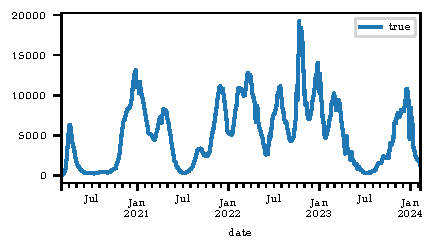
\includegraphics{plots/covid_nowcast/00_true_data.pdf}
    \caption{Realisations.}
    \label{fig:app-covid-true}
    \end{subfigure}\hfill
    \begin{subfigure}[t]{0.48\textwidth}
    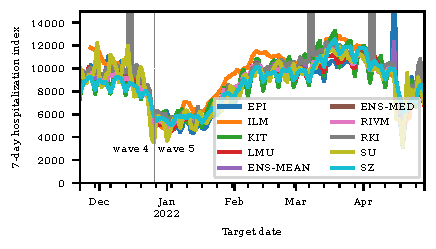
\includegraphics{plots/covid_nowcast/00_nowcast_data.pdf}
    \caption{Same-day nowcasts}
    \label{fig:app-covid-nowcast}
        \end{subfigure}
    \caption{True and nowcast data of the seven-day-hospitalization in Germany from November 22, 2021 to April 29, 2022 \parencite{ChairOfEconometricsAndStatisticsAtKarlsruheInstituteOfTechnology2024}.
    The outliers in the RKI model of values above $10^8$ are removed before the following analysis.}
    \label{fig:app-covid-true-nowcast}
\end{figure}


The data contains 8 nowcasts from scientific and public institutions, nowcast communities and a newspaper, using different input variables, calendar data, and length of training data.
The model structures are diverse, including bayesian models, generalized additive models, and parametric bootstrapping.
Table~\ref{tab:app-covid-models} in the appendix lists the different abbreviations and the overall structure of the model.
Using the nowcasts, two ensemble methods are constructed by using mean or median of the ensembles.
We denote them by ENS-MEAN and ENS-MED.
In line with the initial study design, we consider the time span from November 22, 2021 to April 29, 2022 as evaluation period.
In contrast to~\textcite{Wolffram2023} we use the newest data available on the true values and not the data from August 8, 2022.
\unsure{Nochmal längere Evaluation?}
We do not expand on the models' performance on specific regions or age groups in Germany and on the probabilistic nowcast assessment.
Figure~\ref{fig:app-covid-true-nowcast} displays the true and nowcast data for the evaluation period.
The time comprises the forth wave's end in December 2021 and nearly the entire fifth wave of the pandemic in Germany lasting until May 28, 2022~\parencite{Tolksdorf2022}.
Table~\ref{tab:app-covid-rmse} summarizes the point evaluation measures for the issued mean of the different models.
The models issue same-day nowcasts for nearly all 159 days of the evaluation period~\parencite[see][Tables A2, A3, and A4]{Wolffram2023}.
The best performing models are the ILM and RKI model in terms of both RMSE and MAE.
The ensemble methods perform worse than the best models in terms of the mean location.
The performance of the models is diverse, with more than twice as high RMSE values for the worst models compared to the best models.
Note that the high values for the EPI model could be driven by a very far off value at the end of the evaluation period.

In addition to close inspection of the point evaluation measures, assessing trending of the nowcasts is crucial.
To assess the impact of taken measures and the direction of curve, it is important to distinguish between rising and falling hospitalization rates.
If hospitalization rates are rising, measures should be tightened, while falling rates might allow for loosening measures.
Especially, asymmetries are of interest: Are some models better in recognizing a fall than a rise or vice versa?

In the following, we apply the trending assessment of Section~\ref{sec:trending} to the nowcasts of the seven-day hospitalization rate.
We report the trending for the lags 1, 7, and 14 days.
While lag 1 assesses the short-term trending, lags 7 and 14 assess the medium-term trending.
For the best models in terms of point evaluation, we also assess the trending with the conditional probability plot.

\begin{table}[]
    \centering
    \begin{tabular}{llllr}
\toprule
 & rmse & mae & mse & count \\
model &  &  &  &  \\
\midrule
ILM-prop & :,.f & :,.f & :,.f & 530 \\
RIVM-KEW & :,.f & :,.f & :,.f & 817 \\
NowcastHub-MeanEnsemble & :,.f & :,.f & :,.f & 610 \\
NowcastHub-MedianEnsemble & :,.f & :,.f & :,.f & 610 \\
LMU_StaBLab-GAM_nowcast & :,.f & :,.f & :,.f & 574 \\
RKI-weekly_report & :,.f & :,.f & :,.f & 334 \\
KIT-simple_nowcast & :,.f & :,.f & :,.f & 861 \\
SZ-hosp_nowcast & :,.f & :,.f & :,.f & 535 \\
SU-hier_bayes & :,.f & :,.f & :,.f & 423 \\
Epiforecasts-independent & :,.f & :,.f & :,.f & 275 \\
\bottomrule
\end{tabular}

    \caption{Point evaluation measures for the issued mean of the different models. The evaluation period comprises 159 days. }
    \label{tab:app-covid-rmse}
\end{table}


\begin{table}
    \centering
    \missingfigure{TABLE}
    \caption{Trending ratios for the models with and without exclusion areas. The exclusion areas are rectangles centered on the zero points with width and height ... . The ratios are calculated for the lags 1, 7, and 14 days.}
    \label{tab:app-covid-ratios}
\end{table}

\newpage
\subsection{Forecasting emergency department arrivals}\label{sec:application-eda}

\textcite{Rostami-Tabar2023}

Paper setup:

\begin{itemize}
    \item (Probabilistic) forecast of the hourly number of arrivals in large emergency department (take expectation as point forecast)
    \item Forecasts are produced 48 hours ahead on a 12-hour-rolling basis; background: \enquote{It enables planners to match ED staff to the number of arrivals, redeploy staff, and reconfigure units.}
    \item training data: 2014-04-01 to 2018-2-28
    \item evaluation from 2018-03-01 to 2019-02-28
    \item Evaluation in Paper through RMSE; Pinball Loss and PIT-histograms
    \item consider several lags:
    \begin{itemize}
        \item 72-hours-lag: Is the forecast showing the correct change compared to the most recent observation (problem: strong weekly structure (i.e., Monday and Saturday highest) makes it easy to predict right direction)
        \item 7-days-lag: Correct trend compared to the last shift of same hour and day $\rightarrow$ change policies compared to that
        \item Take first issued forecast for every target time
    \end{itemize}
\end{itemize}

\begin{table}
\centering
\begin{tabular}{llll}
\toprule
 & trend acc lag 3d & trend acc lag 7d & rmse \\
\midrule
Benchmark-1 & 0.7867 & 0.7556 & 10.0654 \\
Benchmark-2 & 0.7847 & 0.7615 & 9.2462 \\
Poisson-1 & 0.7876 & 0.7661 & 9.1639 \\
Poisson-2 & 0.7886 & 0.7655 & 8.8838 \\
NOtr-1 & 0.7829 & 0.7609 & 9.4132 \\
NOtr-2 & 0.7829 & 0.7609 & 9.4132 \\
GBM-2 & 0.7697 & 0.7413 & 11.6628 \\
Ttr-2 & 0.7857 & 0.7651 & 9.3944 \\
NBI-2 & 0.7895 & 0.7656 & 8.8829 \\
qreg-1 & 0.7501 & 0.7291 & 13.3367 \\
Poisson-2-I & 0.7834 & 0.7615 & 9.4579 \\
tbats & 0.6906 & 0.6659 & 12.9049 \\
ADAM-iETSX & 0.6794 & 0.6633 & 28.0003 \\
ETS & 0.6561 & 0.6471 & 29.3577 \\
Regression-Poisson & 0.6930 & 0.6742 & 21.1623 \\
Prophet & 0.6864 & 0.6724 & 13.0785 \\
\bottomrule
\end{tabular}

\caption{Accuracies (without exclusion area) and RMSE for the considered models in \textcite{Rostami-Tabar2023}}	
\end{table}

\begin{figure}
	\centering
	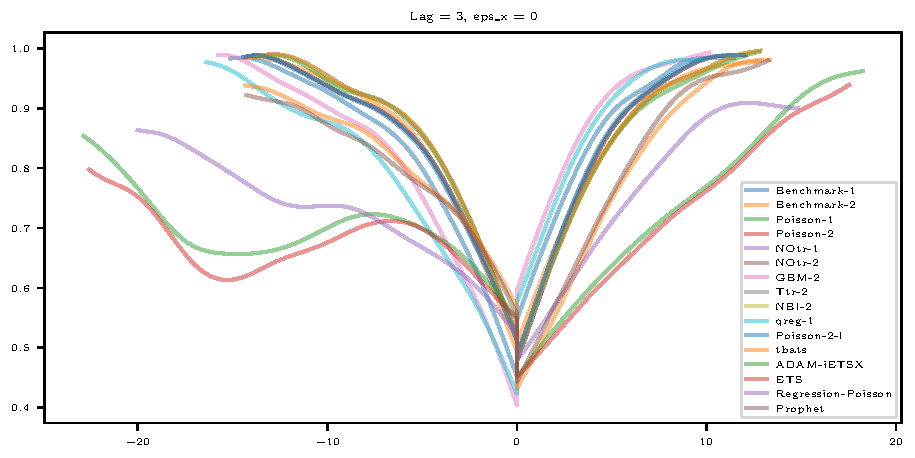
\includegraphics{plots/ed_arrival/Cond_Prob_lag_3.pdf}
        \caption{Conditional probability plot for ED arrival}
\end{figure}